\section{Thống kê suy diễn}
    \subsection{Phân tích phương sai một nhân tố (ANOVA) và hậu kiểm theo nhà sản xuất}
    \textbf{Bài toán:} Trên thị trường card đồ họa hiện nay, có 4 nhãn hàng chính cạnh tranh với nhau là \textbf{AMD}, \textbf{ATI}, \textbf{Intel} và \textbf{Nvidia}. Tốc độ xung nhịp nhân (\texttt{Core\_Speed}, đơn vị: MHz) là một trong những thông số cốt lõi phản ánh năng lực xử lý của GPU. Với mức ý nghĩa $\alpha = 0.05$, hãy đánh giá xem nhà sản xuất (\texttt{Manufacturer}) có ảnh hưởng đến tốc độ xung nhịp nhân trung bình của GPU hay không.

    \subsubsection{Thống kê mô tả và xây dựng giả thuyết}
        Sau khi chuẩn hóa dữ liệu và loại bỏ trùng lặp theo tên từng mẫu GPU (\texttt{Name}), bộ dữ liệu thu được $N = 2,469$ mẫu GPU thuộc 4 nhà sản xuất, trong đó cỡ mẫu của từng nhóm đều lớn hơn $30$ ($n_i \ge 80$), đảm bảo điều kiện áp dụng Định lý Giới hạn Trung tâm:

        \begin{table}[H]
            \centering
            \renewcommand{\arraystretch}{1.3}
            \begin{tabular}{|l|r|r|r|r|r|}
                \hline
                \textbf{Nhà sản xuất} & \textbf{Số lượng ($n$)} & \textbf{Trung bình (Mean)} & \textbf{Độ lệch chuẩn (SD)} & \textbf{Trung vị (Median)} & \textbf{IQR} \\
                \hline
                \texttt{AMD} & 852 & 896.41 & 166.57 & 925.00 & 218.00 \\
                \hline
                \texttt{ATI} & 80 & 1076.53 & 83.40 & 1120.00 & 30.00 \\
                \hline
                \texttt{Intel} & 115 & 355.05 & 153.24 & 300.00 & 50.00 \\
                \hline
                \texttt{Nvidia} & 1422 & 1017.59 & 276.57 & 1006.00 & 355.00 \\
                \hline
            \end{tabular}
            \caption{Thống kê mô tả biến \texttt{Core\_Speed} (MHz) theo từng nhà sản xuất}
            \label{tab:anova_desc}
        \end{table}

        Gọi $\mu_{\text{AMD}}, \mu_{\text{ATI}}, \mu_{\text{Intel}}, \mu_{\text{Nvidia}}$ lần lượt là tốc độ xung nhịp nhân trung bình của GPU thuộc 4 nhà sản xuất. Ta thiết lập cặp giả thuyết kiểm định:
        \begin{itemize}
            \item $H_0: \mu_{\text{AMD}} = \mu_{\text{ATI}} = \mu_{\text{Intel}} = \mu_{\text{Nvidia}}$ (Không có sự khác biệt về tốc độ xung nhịp nhân trung bình giữa các nhà sản xuất).
            \item $H_1:$ Tồn tại ít nhất hai nhà sản xuất có tốc độ xung nhịp nhân trung bình khác nhau.
        \end{itemize}

    \subsubsection{Kiểm tra các giả định của mô hình ANOVA}
        \begin{enumerate}
            \item \textbf{Tính độc lập của các quan sát:} Các mẫu GPU trong bộ dữ liệu đại diện cho từng dòng sản phẩm độc lập sau khi đã lọc trùng theo tên sản phẩm, do đó giả định độc lập được thỏa mãn.
            \item \textbf{Kiểm định phân phối chuẩn (Shapiro-Wilk Test):}
            \begin{itemize}
                \item Kết quả kiểm định Shapiro-Wilk trên cả 4 nhóm đều cho $\text{p-value} < 0.05$ ($\text{AMD}: W = 0.967, p = 6.14 \times 10^{-13}$; $\text{ATI}: W = 0.709, p = 2.70 \times 10^{-11}$; $\text{Intel}: W = 0.686, p = 2.35 \times 10^{-14}$; $\text{Nvidia}: W = 0.976, p = 1.71 \times 10^{-14}$).
                \item Tuy nhiên, vì kích thước mẫu của cả 4 nhóm đều lớn ($n_{\min} = 80 > 30$), theo Định lý Giới hạn Trung tâm, phân phối của trung bình mẫu tiệm cận phân phối chuẩn nên phương pháp ANOVA vẫn đảm bảo tính vững (robustness).
            \end{itemize}
            \item \textbf{Kiểm định tính đồng nhất phương sai (Levene's Test):}
            \begin{itemize}
                \item Giả thuyết $H_0$: Phương sai của \texttt{Core\_Speed} giữa 4 nhà sản xuất là bằng nhau ($\sigma_1^2 = \sigma_2^2 = \sigma_3^2 = \sigma_4^2$).
                \item Kết quả kiểm định Levene cho thống kê $F = 83.664$ với $\text{p-value} < 2.2 \times 10^{-16} < 0.05 \Rightarrow$ Bác bỏ $H_0$. Như vậy, phương sai giữa các nhóm là \textbf{không đồng nhất}.
                \item Để đảm bảo tính chính xác tuyệt đối khi giả định đồng nhất phương sai bị vi phạm, nhóm thực hiện song song cả \textbf{ANOVA tiêu chuẩn} và kiểm định hiệu chỉnh \textbf{Welch's ANOVA} (\texttt{oneway.test(..., var.equal = FALSE)}).
            \end{itemize}
        \end{enumerate}
        \begin{figure}[H]
            \centering
            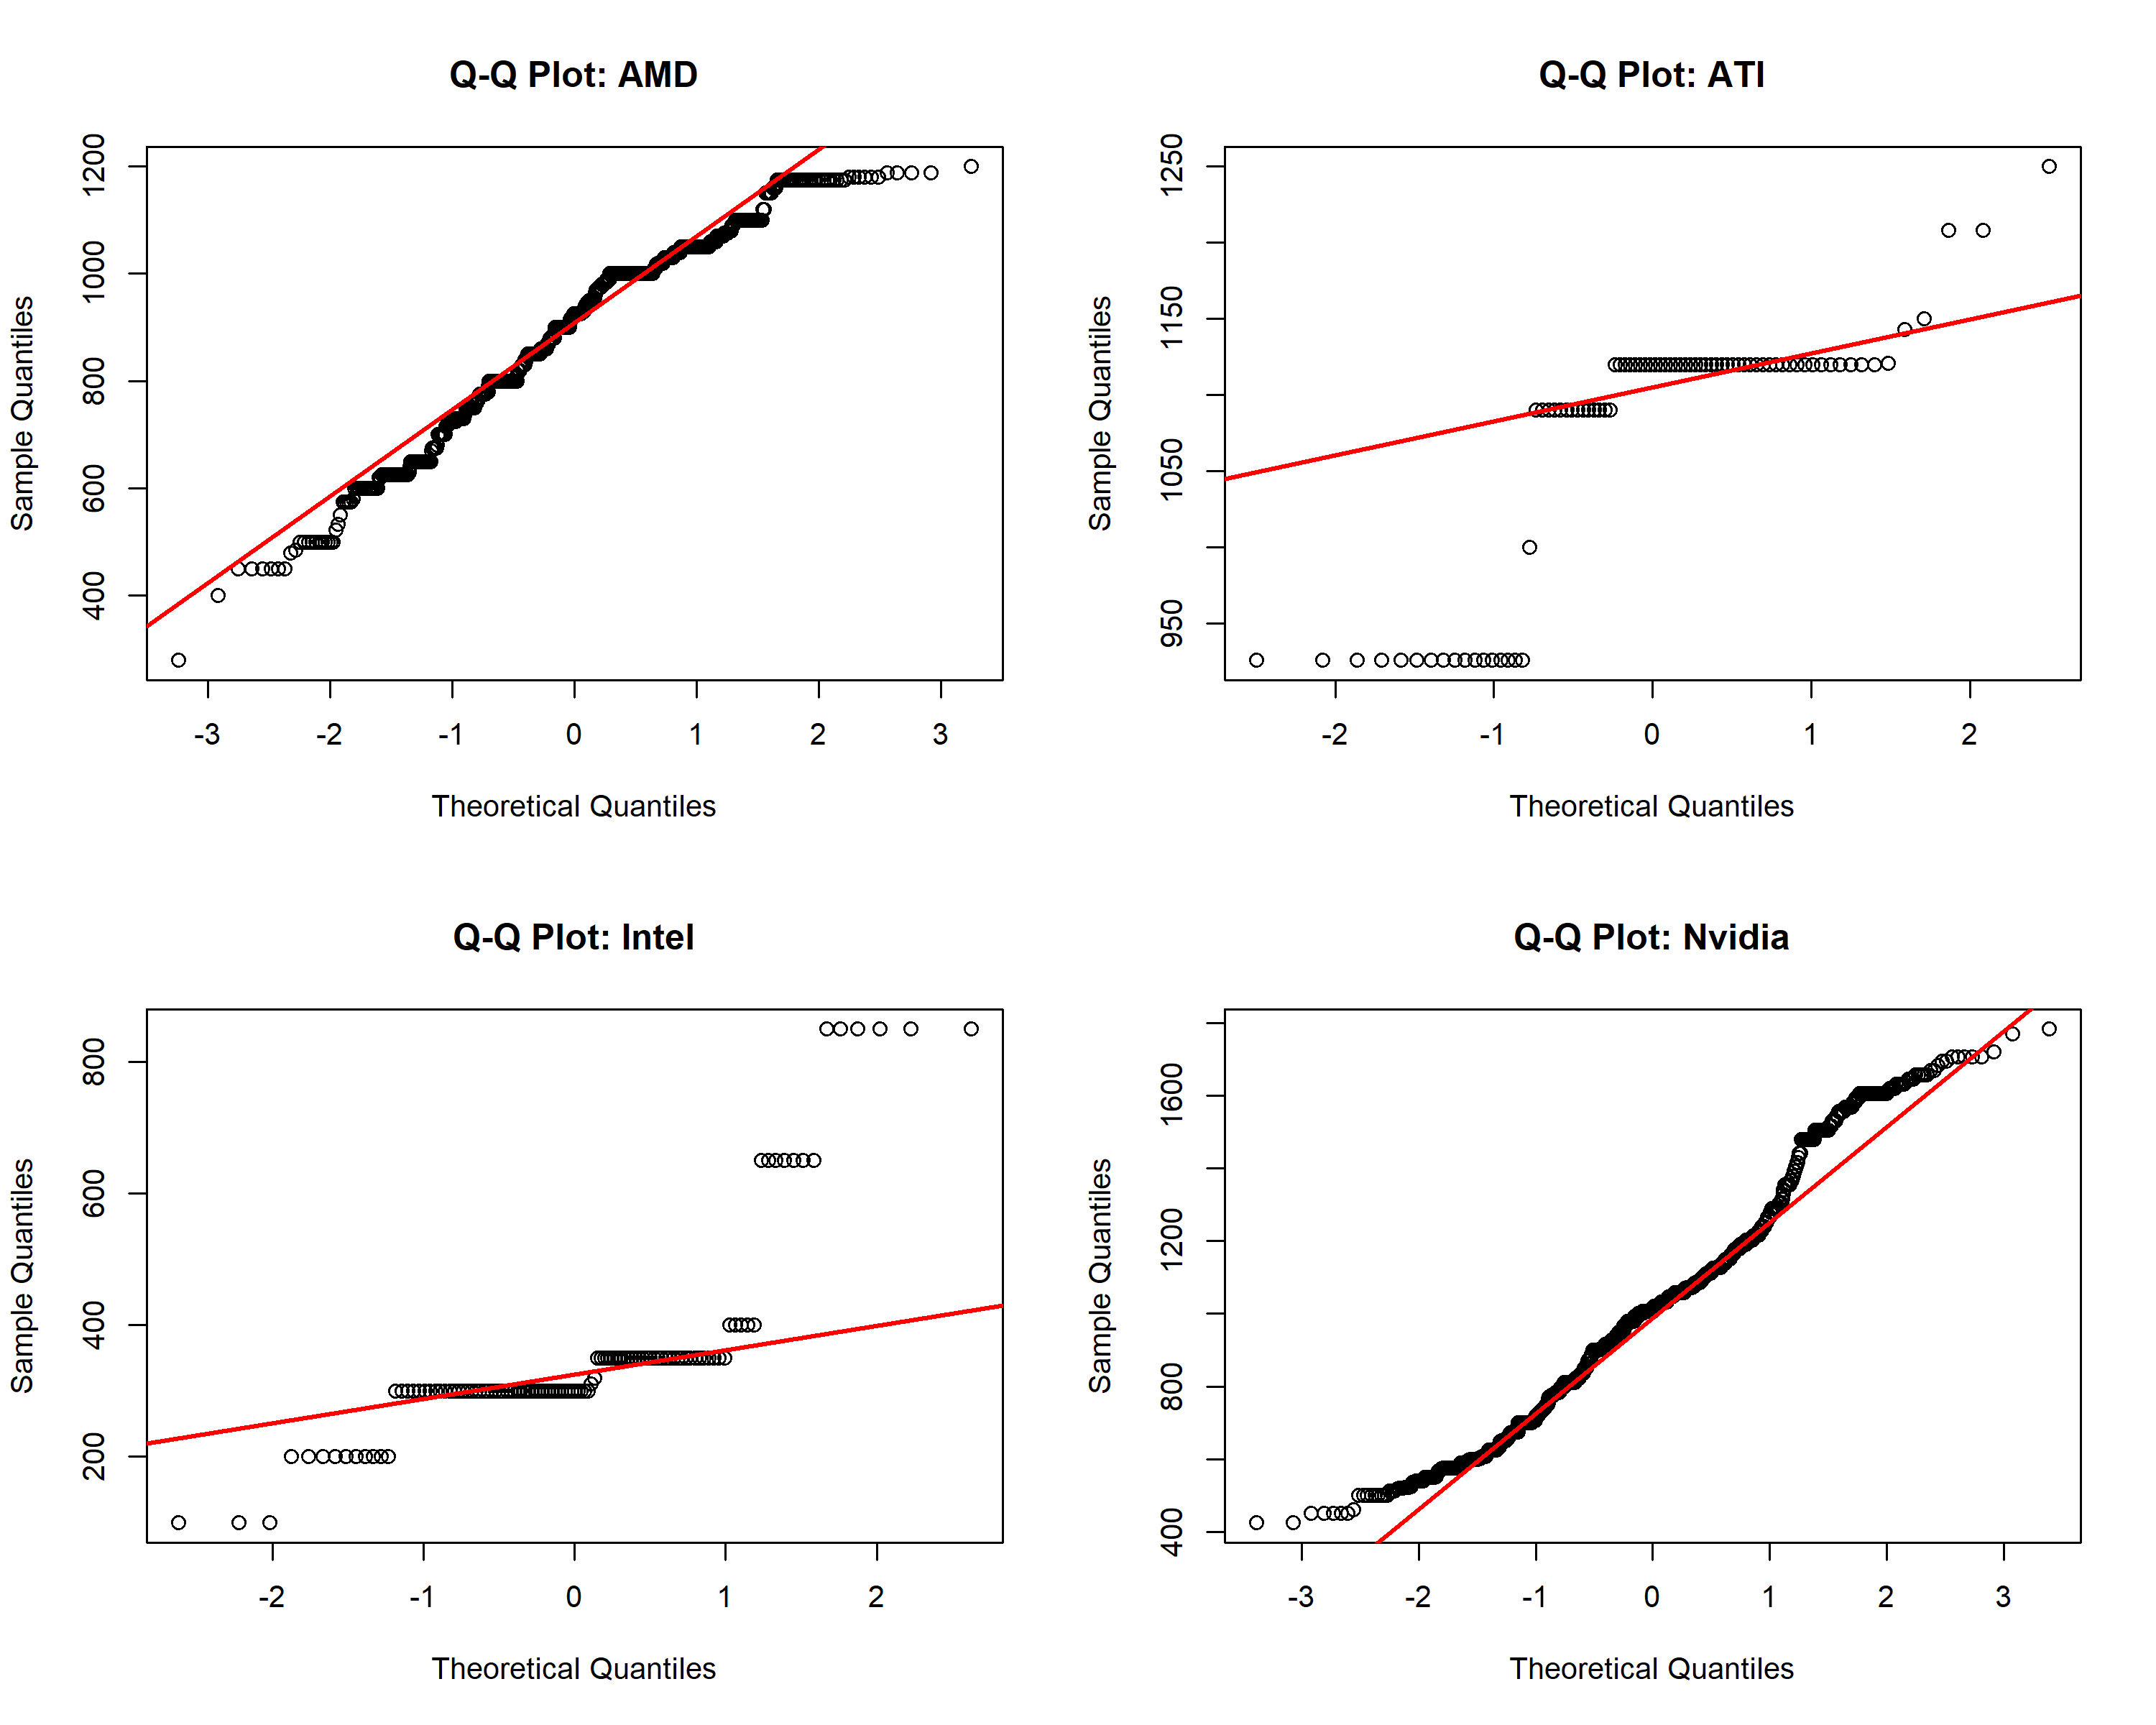
\includegraphics[width=0.9\textwidth]{statisticPros/anova_qqplot.png}
            \caption{Biểu đồ Q-Q Plot kiểm tra phân phối chuẩn của \texttt{Core\_Speed} theo 4 nhà sản xuất}
            \label{fig:anova_qqplot}
        \end{figure}
        
        \begin{figure}[H]
            \centering
            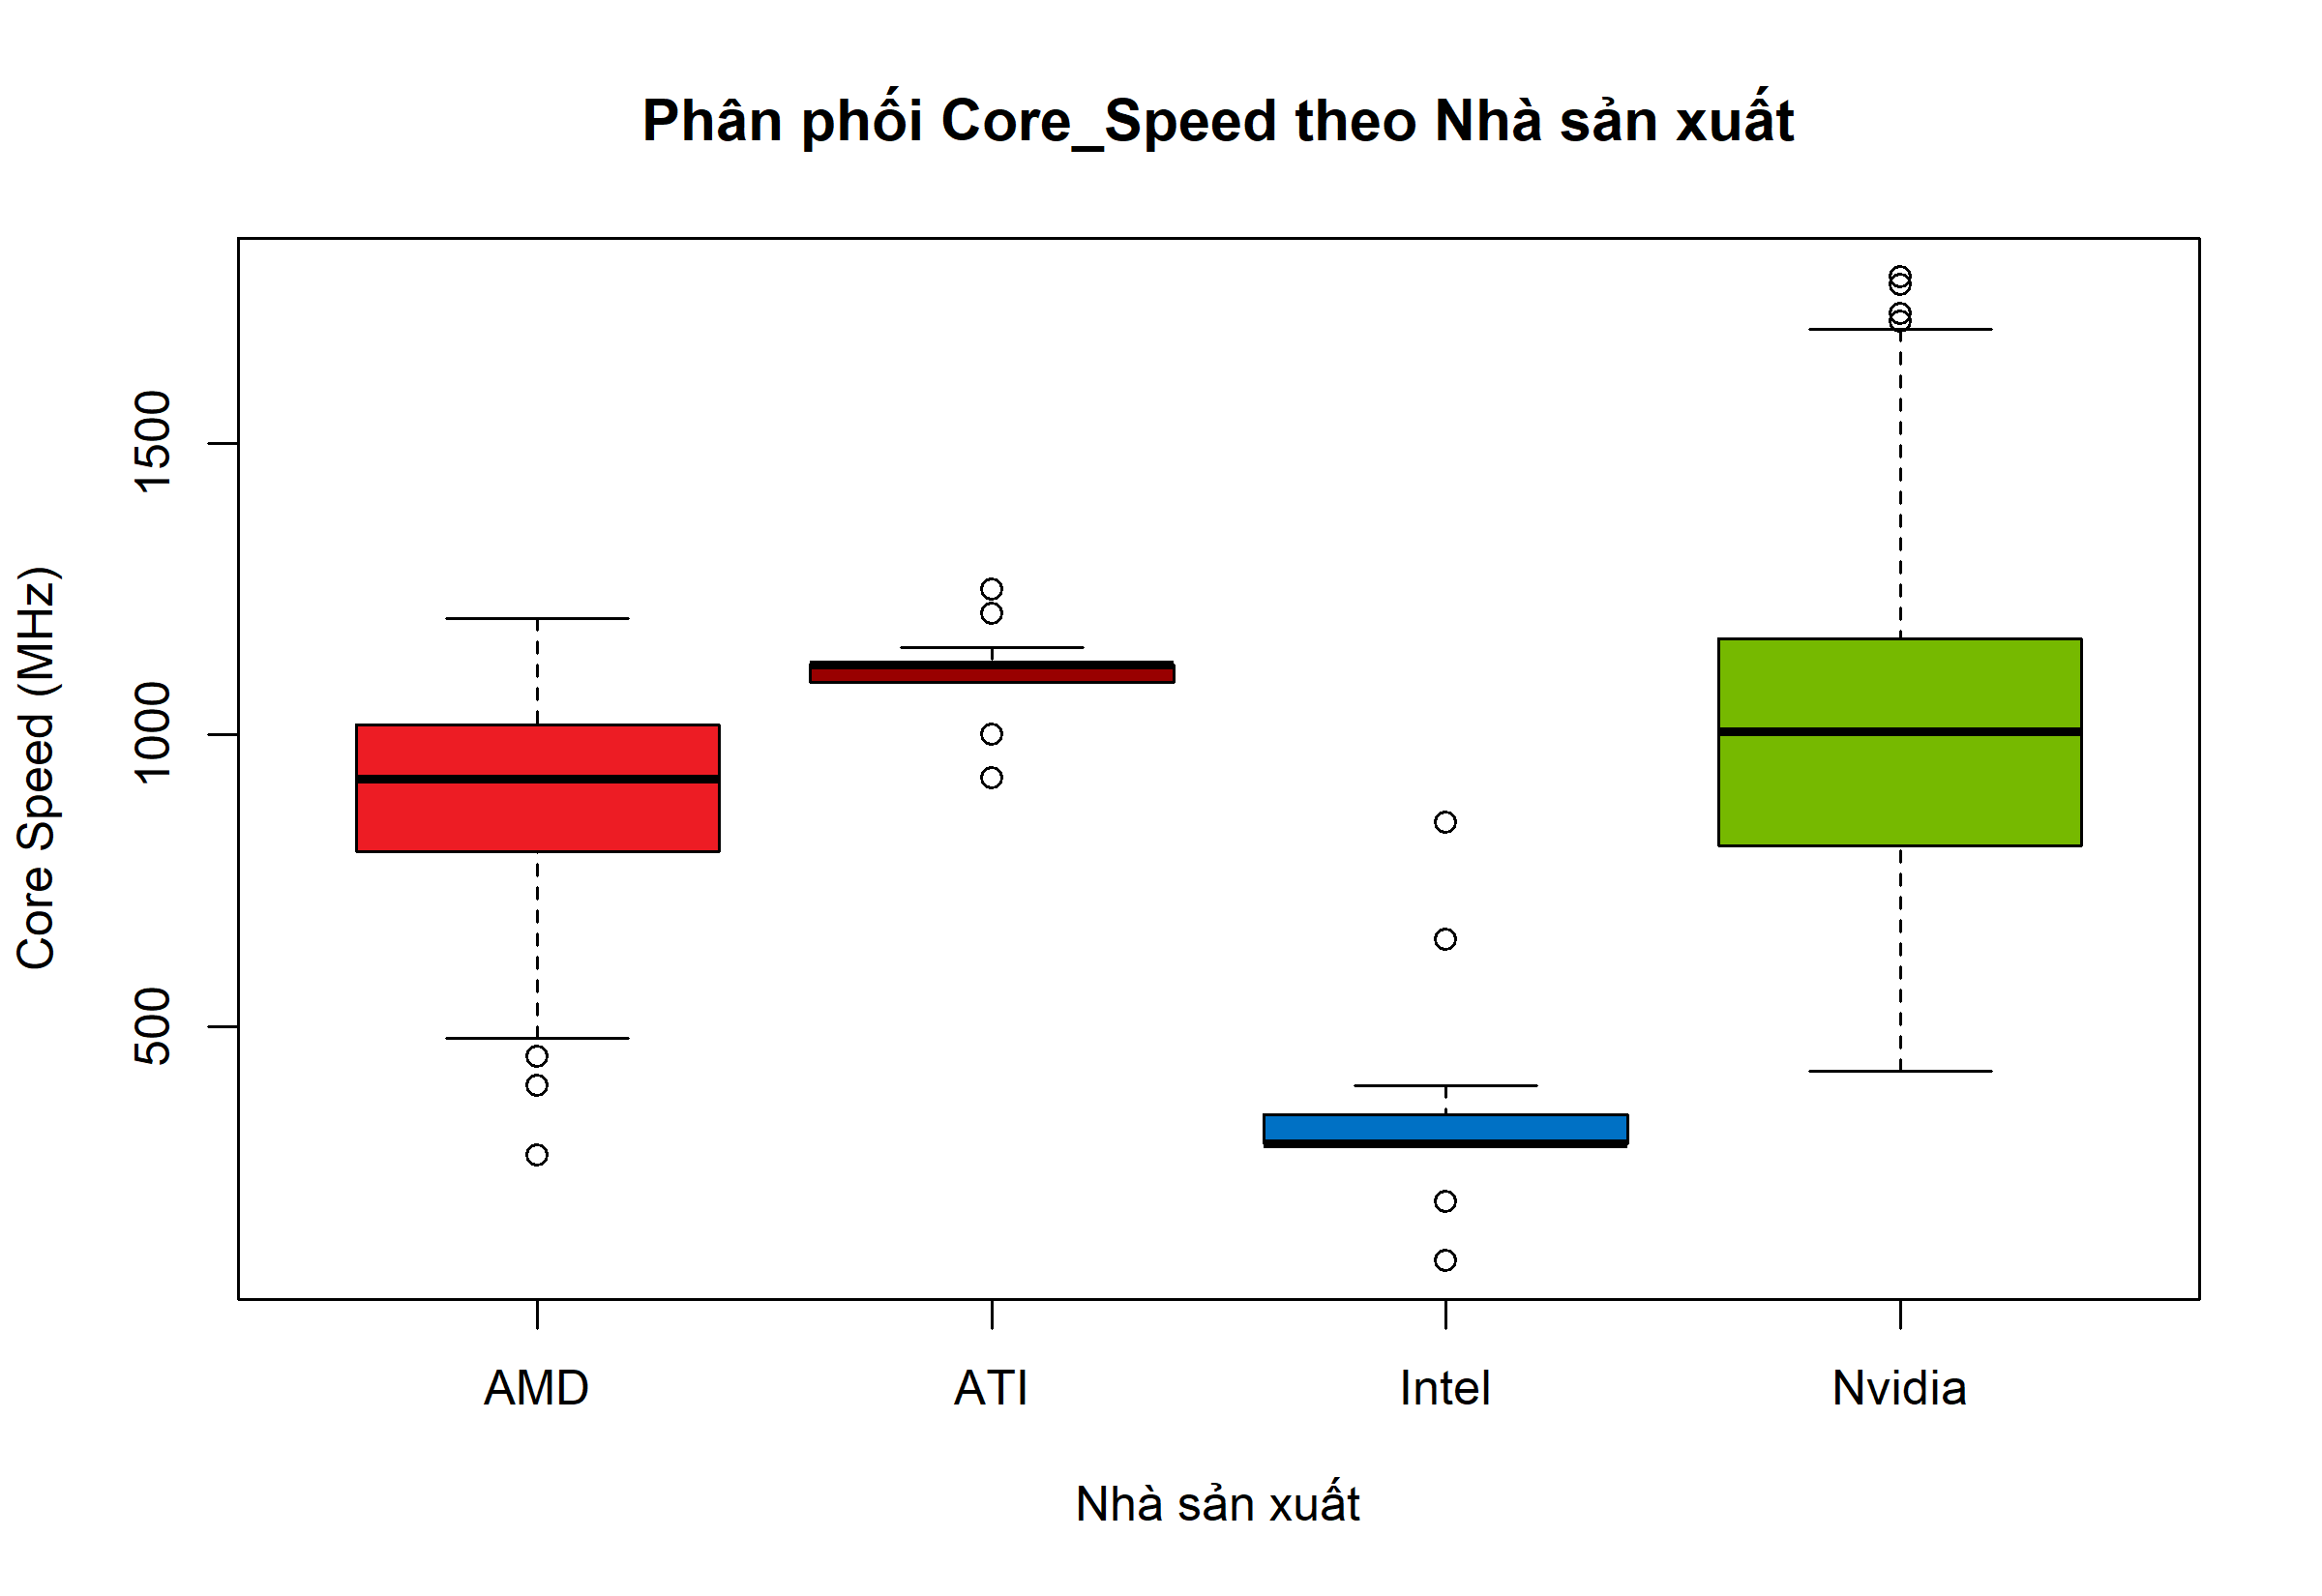
\includegraphics[width=0.82\textwidth]{statisticPros/anova_boxplot.png}
            \caption{Biểu đồ Boxplot so sánh phân phối \texttt{Core\_Speed} giữa các nhà sản xuất}
            \label{fig:anova_boxplot}
        \end{figure}


    \subsubsection{Kết quả mô hình ANOVA và phân tích hậu kiểm (Post-hoc)}
        \textbf{1. Kết quả kiểm định ANOVA:}
        \begin{itemize}
            \item \textbf{ANOVA tiêu chuẩn:} Thống kê $F(3, 2465) = 308.6$, $\text{p-value} < 2 \times 10^{-16} < \alpha = 0.05$.
            \item \textbf{Welch's ANOVA (không giả định phương sai bằng nhau):} Thống kê $F(3, 297.24) = 676.55$, $\text{p-value} < 2.2 \times 10^{-16} < \alpha = 0.05$.
            \item $\Rightarrow$ Cả hai phương pháp đều dẫn đến quyết định \textbf{bác bỏ $H_0$}. Có sự khác biệt có ý nghĩa thống kê rất cao về tốc độ xung nhịp nhân trung bình giữa các nhà sản xuất GPU.
        \end{itemize}

        \textbf{2. Phân tích hậu kiểm Tukey HSD (So sánh bội từng cặp):}
        \begin{table}[H]
            \centering
            \renewcommand{\arraystretch}{1.3}
            \begin{tabular}{|l|r|r|r|r|l|}
                \hline
                \textbf{Cặp so sánh} & \textbf{Chênh lệch (diff)} & \textbf{Cận dưới (lwr)} & \textbf{Cận trên (upr)} & \textbf{$p_{\text{adj}}$} & \textbf{Kết luận ($\alpha = 0.05$)} \\
                \hline
                \texttt{ATI - AMD} & $+180.11$ & $+109.62$ & $+250.60$ & $0.0000$ & Khác biệt có ý nghĩa \\
                \hline
                \texttt{Intel - AMD} & $-541.36$ & $-601.25$ & $-481.47$ & $0.0000$ & Khác biệt có ý nghĩa \\
                \hline
                \texttt{Nvidia - AMD} & $+121.17$ & $+95.06$ & $+147.29$ & $0.0000$ & Khác biệt có ý nghĩa \\
                \hline
                \texttt{Intel - ATI} & $-721.47$ & $-809.23$ & $-633.71$ & $0.0000$ & Khác biệt có ý nghĩa \\
                \hline
                \texttt{Nvidia - ATI} & $-58.94$ & $-128.21$ & $+10.33$ & $0.1269$ & \textbf{Không có sự khác biệt} \\
                \hline
                \texttt{Nvidia - Intel} & $+662.53$ & $+604.09$ & $+720.97$ & $0.0000$ & Khác biệt có ý nghĩa \\
                \hline
            \end{tabular}
            \caption{Kết quả kiểm định hậu kiểm Tukey HSD giữa các cặp nhà sản xuất}
            \label{tab:tukey_hsd}
        \end{table}

        \textbf{Kết luận rút ra từ mô hình ANOVA:}
        \begin{itemize}
            \item \textbf{Nhóm hiệu năng xung nhịp cao (\texttt{ATI} và \texttt{Nvidia}):} Hai hãng này dẫn đầu về tốc độ xung nhịp nhân trung bình (lần lượt là $1076.53\text{ MHz}$ và $1017.59\text{ MHz}$). Đặc biệt, phép kiểm định hậu kiểm cho thấy giữa \texttt{Nvidia} và \texttt{ATI} \textbf{không có sự khác biệt có ý nghĩa thống kê} về tốc độ xung nhịp trung bình ($p_{\text{adj}} = 0.1269 > 0.05$).
            \item \textbf{Nhóm tầm trung (\texttt{AMD}):} Có tốc độ xung nhịp trung bình đạt $896.41\text{ MHz}$, thấp hơn đáng kể so với \texttt{ATI} ($-180.11\text{ MHz}$) và \texttt{Nvidia} ($-121.17\text{ MHz}$).
            \item \textbf{Nhóm xung nhịp thấp (\texttt{Intel}):} Có tốc độ xung nhịp trung bình thấp nhất ($355.05\text{ MHz}$), chênh lệch rất lớn so với cả 3 hãng còn lại ($p_{\text{adj}} < 0.0001$). Điều này hoàn toàn phù hợp với thực tế công nghệ vì đa số GPU của Intel trong tập dữ liệu là chip đồ họa tích hợp (iGPU) tối ưu cho tiết kiệm điện năng, trong khi AMD, ATI và Nvidia tập trung vào dòng card đồ họa rời (dGPU) hiệu năng cao.
        \end{itemize}


    \subsection{Mô hình hồi quy tuyến tính}
        Phân tích hồi quy tuyến tính bội (Multiple Linear Regression) là phương pháp thống kê nhằm xác định mối quan hệ tuyến tính giữa một biến phụ thuộc $Y$ với nhiều biến độc lập $X_1, X_2, \dots, X_n$, từ đó dự đoán giá trị của $Y$ khi các biến độc lập thay đổi. Phương trình tổng quát có dạng:
        \[Y = w_0 + w_1X_1 + w_2X_2 + \dots + w_nX_n + \varepsilon\]
        Trong phương trình hồi quy tuyến tính đa biến có những yếu tố sau:
        \begin{itemize}
            \item $Y$: Biến phụ thuộc (giá trị đầu ra cần dự đoán của mô hình).
            \item $X_1, X_2, \dots, X_n$: Các biến độc lập (các biến đầu vào của mô hình).
            \item $w_0$: Hệ số chặn (Intercept).
            \item $w_1, w_2, \dots, w_n$: Các trọng số (hệ số hồi quy), thể hiện mức độ ảnh hưởng của từng biến đầu vào đến kết quả dự đoán.
            \item $\varepsilon$: Sai số ngẫu nhiên, thể hiện phần biến thiên của giá trị thực tế mà mô hình chưa giải thích được.
        \end{itemize}

    \subsection{Mục tiêu và phương pháp xây dựng mô hình}
        \subsubsection{Mô hình 1}
            Ở mô hình này, ta phân tích sự tác động của 7 yếu tố phần cứng gồm: \texttt{Memory\_Bandwidth}, \texttt{Memory}, \texttt{Memory\_Speed}, \texttt{Memory\_Bus}, \texttt{Process}, \texttt{ROPs}, \texttt{TMUs} lên \texttt{Core\_Speed} (chưa xét đến công suất tiêu thụ tối đa).
            \begin{itemize}
                \item \textbf{Biến phụ thuộc:} \texttt{Core\_Speed}
                \item \textbf{Biến độc lập:} \texttt{Memory\_Bandwidth}, \texttt{Memory}, \texttt{Memory\_Speed}, \texttt{Memory\_Bus}, \texttt{Process}, \texttt{ROPs}, \texttt{TMUs}
            \end{itemize}
            Phương trình biểu diễn mô hình:
            \[\texttt{Core\_Speed} = w_0 + w_1X_1 + w_2X_2 + \dots + w_7X_7 + \varepsilon\]

        \subsubsection{Mô hình 2}
            Mô hình 2 khảo sát sự tác động khi lược bỏ bớt biến tốc độ bộ nhớ (\texttt{Memory\_Speed}) và công suất (\texttt{Max\_Power}), giữ lại 6 biến độc lập: \texttt{Memory\_Bandwidth}, \texttt{Memory}, \texttt{Memory\_Bus}, \texttt{Process}, \texttt{ROPs}, \texttt{TMUs}.
            \begin{itemize}
                \item \textbf{Biến phụ thuộc:} \texttt{Core\_Speed}
                \item \textbf{Biến độc lập:} \texttt{Memory\_Bandwidth}, \texttt{Memory}, \texttt{Memory\_Bus}, \texttt{Process}, \texttt{ROPs}, \texttt{TMUs}
            \end{itemize}

        \subsubsection{Mô hình 3 (Mô hình dạng Logarit đầy đủ)}
            Ở mô hình chính này, ta áp dụng phép biến đổi logarit tự nhiên ($\ln$) cho toàn bộ biến phụ thuộc và đầy đủ 8 biến độc lập để tuyến tính hóa mối quan hệ và ổn định phương sai:
            \begin{itemize}
                \item \textbf{Biến phụ thuộc:} $\log(\texttt{Core\_Speed})$
                \item \textbf{Biến độc lập:} $\log(\texttt{Max\_Power})$, $\log(\texttt{Memory\_Bandwidth})$, $\log(\texttt{Memory})$, $\log(\texttt{Memory\_Speed})$, $\log(\texttt{Memory\_Bus})$, $\log(\texttt{Process})$, $\log(\texttt{ROPs})$, $\log(\texttt{TMUs})$
            \end{itemize}

            \textbf{Mã nguồn R xây dựng và tóm tắt Mô hình 3:}
\begin{pythoncode}
Model3 <- lm(Core_Speed ~ Max_Power + Memory_Bandwidth + Memory + Memory_Speed + 
               Memory_Bus + Process + ROPs + TMUs, data = df_log)
print(summary(Model3))
\end{pythoncode}

            \begin{figure}[H]
                \centering
                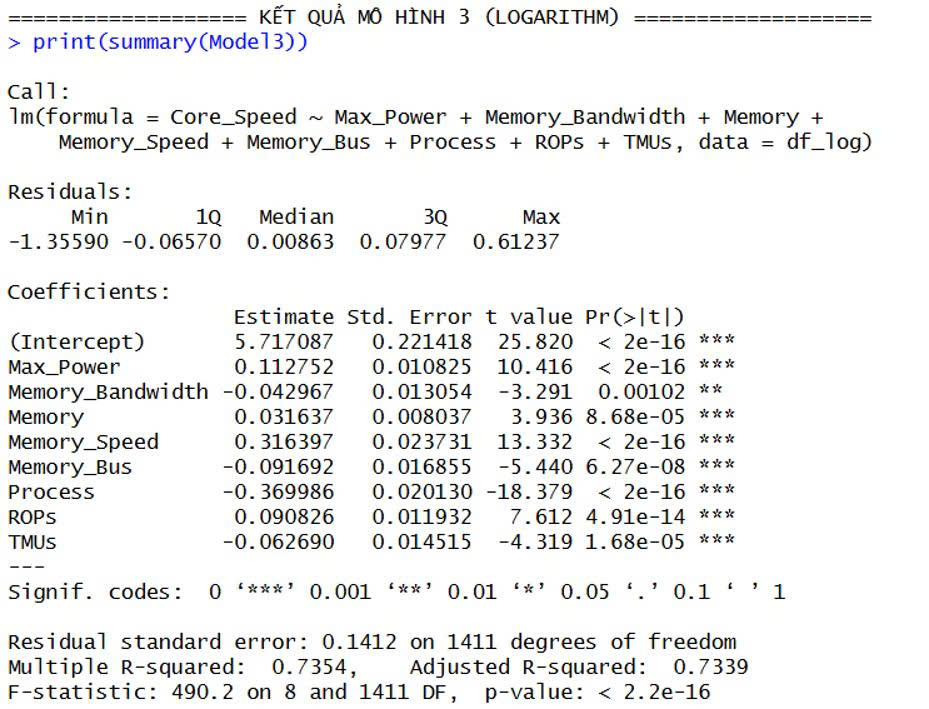
\includegraphics[width=0.92\textwidth]{statisticPros/model3_summary.jpg}
                \caption{Kết quả hồi quy tuyến tính bội của Mô hình 3 trong R}
                \label{fig:model3_summary}
            \end{figure}

    \subsection{Phân tích sự tác động của các yếu tố lên hiệu năng GPUs}
        Từ bảng kết quả ước lượng của Mô hình 3 (Hình \ref{fig:model3_summary}), phương trình hồi quy tuyến tính biểu diễn ảnh hưởng của các nhân tố đến xung nhịp nhân \texttt{Core\_Speed} của GPU có dạng:
        \begin{align*}
            \log(\texttt{Core\_Speed}) &= 5.717087 + 0.112752 \times \log(\texttt{Max\_Power}) - 0.042967 \times \log(\texttt{Memory\_Bandwidth}) \\
            &\quad + 0.031637 \times \log(\texttt{Memory}) + 0.316397 \times \log(\texttt{Memory\_Speed}) \\
            &\quad - 0.091692 \times \log(\texttt{Memory\_Bus}) - 0.369986 \times \log(\texttt{Process}) \\
            &\quad + 0.090826 \times \log(\texttt{ROPs}) - 0.062690 \times \log(\texttt{TMUs})
        \end{align*}

        \textbf{Đánh giá chi tiết mô hình:}
        \begin{itemize}
            \item \textbf{Kiểm định sự phù hợp chung (F-test):} Giá trị thống kê $F = 490.2$ (với bậc tự do $8$ và $1411$) có giá trị $\text{p-value} < 2.2 \times 10^{-16}$, nhỏ hơn rất nhiều so với mức ý nghĩa $\alpha = 0.05$ (thậm chí nhỏ hơn mức $0.001$). Điều này chứng tỏ mô hình hồi quy xây dựng được là rất phù hợp và các biến độc lập có ý nghĩa giải thích rất cao cho biến phụ thuộc \texttt{Core\_Speed}.
            \item \textbf{Đánh giá ý nghĩa thống kê của từng biến độc lập (t-test):} Xét cột trọng số (\texttt{Estimate}) và giá trị $\text{p-value}$ ($\Pr(>\vert{}t\vert{})$) tương ứng, tất cả 8 biến độc lập đều có $\text{p-value}$ rất nhỏ:
            \begin{itemize}
                \item Biến \texttt{Memory\_Bandwidth} có $\text{p-value} = 0.00102$ (đạt mức ý nghĩa $0.01$ — ký hiệu \texttt{**}).
                \item 7 biến còn lại (\texttt{Max\_Power}, \texttt{Memory}, \texttt{Memory\_Speed}, \texttt{Memory\_Bus}, \texttt{Process}, \texttt{ROPs}, \texttt{TMUs}) đều có $\text{p-value} < 0.0001$ (đạt mức ý nghĩa cực kỳ cao $0.001$ — ký hiệu \texttt{***}).
                \item $\Rightarrow$ Như vậy, cả 8 nhân tố đưa vào mô hình đều có ý nghĩa thống kê rất cao và thực sự tác động đến tốc độ xung nhịp \texttt{Core\_Speed} của GPUs.
            \end{itemize}
            \item \textbf{Mức độ giải thích của mô hình ($R^2$):} Hệ số $R^2$ hiệu chỉnh (\texttt{Adjusted R-squared}) bằng $0.7339$ (và \texttt{Multiple R-squared} bằng $0.7354$), nghĩa là các biến độc lập trong mô hình giải thích được \textbf{73.39\%} sự biến thiên của hiệu năng \texttt{Core\_Speed}.
            \item \textbf{Kết luận chiều hướng tác động:} Qua dấu của các trọng số thu được từ mô hình, ta thấy có sự phân hóa rõ rệt giữa hai nhóm nhân tố:
            \begin{itemize}
                \item \textit{Nhóm tác động đồng biến (hệ số dương):} \texttt{Max\_Power} ($+0.112752$), \texttt{Memory} ($+0.031637$), \texttt{Memory\_Speed} ($+0.316397$) và \texttt{ROPs} ($+0.090826$) — khi các thông số này tăng thì \texttt{Core\_Speed} có xu hướng tăng theo.
                \item \textit{Nhóm tác động nghịch biến (hệ số âm):} \texttt{Memory\_Bandwidth} ($-0.042967$), \texttt{Memory\_Bus} ($-0.091692$), \texttt{Process} ($-0.369986$) và \texttt{TMUs} ($-0.062690$). Đặc biệt biến tiến trình sản xuất (\texttt{Process}) có tác động nghịch biến mạnh nhất, phản ánh đúng thực tế công nghệ rằng tiến trình bán dẫn càng thu nhỏ (số nm giảm) thì xung nhịp nhân GPU càng đạt hiệu năng cao hơn.
            \end{itemize}
        \end{itemize}

    \subsection{Đồ thị biểu thị sai số hồi quy}
        Để kiểm tra các giả định của mô hình hồi quy tuyến tính (tính tuyến tính, kỳ vọng sai số bằng 0, phân phối chuẩn của phần dư và phương sai đồng nhất), nhóm tiến hành phân tích 4 biểu đồ chẩn đoán phần dư:

        \subsubsection{Biểu đồ Residuals vs Fitted (Giá trị dư theo giá trị dự đoán)}
            \begin{figure}[H]
                \centering
                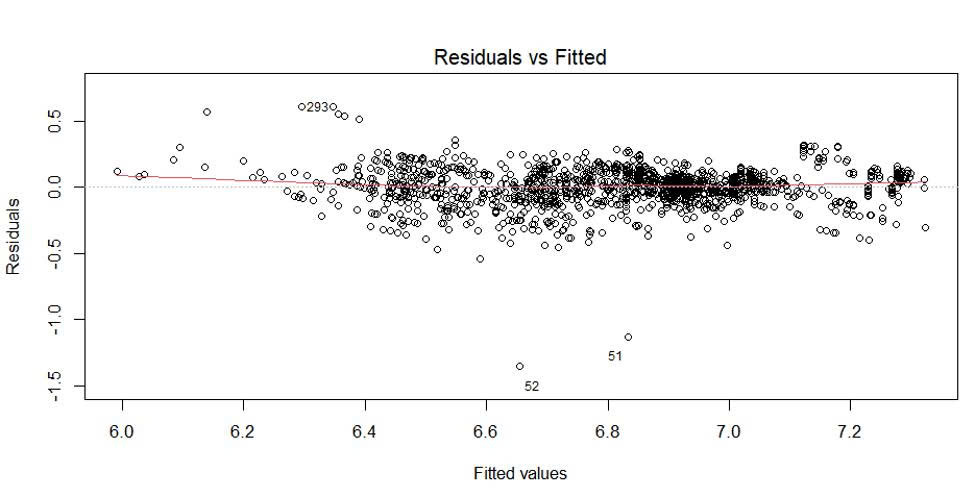
\includegraphics[width=0.88\textwidth]{statisticPros/diag_1_residuals_fitted.jpg}
                \caption{Biểu đồ Residuals vs Fitted}
                \label{fig:res_fitted}
            \end{figure}
            \textbf{Nhận xét:} Đường trung bình (đường màu đỏ) tương đối thẳng, nằm ngang và bám rất sát đường đứt nét $\text{Residuals} = 0$ xuyên suốt miền giá trị dự đoán. Điều này chứng tỏ giả thiết về tính tuyến tính của mô hình và giả thiết kỳ vọng của sai số bằng $0$ đều được thỏa mãn. Các điểm phần dư phân bố ngẫu nhiên quanh đường $0$ và chỉ xuất hiện một vài điểm ngoại lai nhỏ (như điểm 51, 52, 293) không làm ảnh hưởng đến xu hướng chung.

        \subsubsection{Biểu đồ Q-Q Residuals (Kiểm tra phân phối chuẩn)}
            \begin{figure}[H]
                \centering
                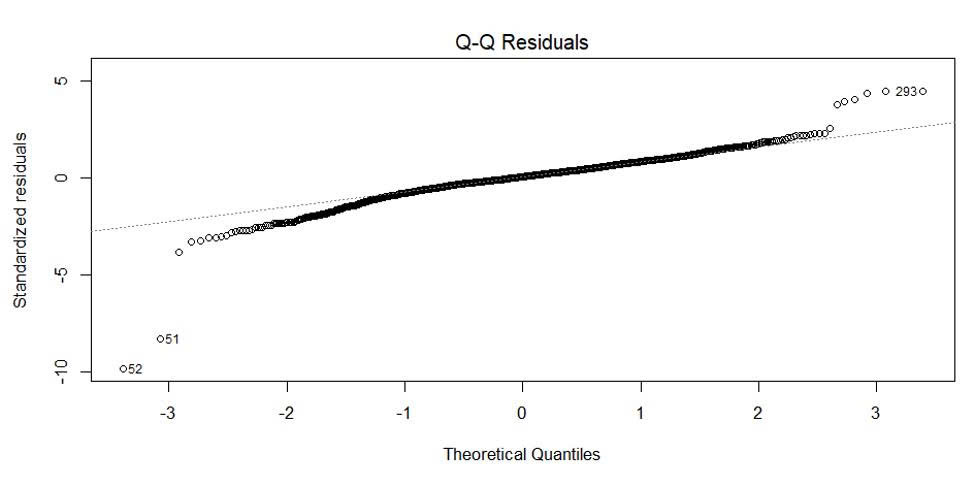
\includegraphics[width=0.88\textwidth]{statisticPros/diag_2_qq.jpg}
                \caption{Biểu đồ Q-Q Residuals}
                \label{fig:qq_res}
            \end{figure}
            \textbf{Nhận xét:} Đa số các điểm phần dư chuẩn hóa nằm bám sát đường thẳng chéo đứt nét trong khoảng giữa (từ $-1.5$ đến $+2.5$), cho thấy phần dư của mô hình nhìn chung tuân theo phân phối chuẩn. Tuy nhiên, ở hai đầu mút vẫn có một số điểm ngoại lai lệch hẳn khỏi đường chuẩn (như điểm 51, 52 lệch xuống dưới ở đuôi trái và điểm 293 lệch lên trên ở đuôi phải), tạo hiện tượng đuôi nặng nhẹ nhưng không làm ảnh hưởng lớn đến tính hợp lệ chung của mô hình do cỡ mẫu lớn.

        \subsubsection{Biểu đồ Scale-Location (Kiểm tra phương sai đồng nhất)}
            \begin{figure}[H]
                \centering
                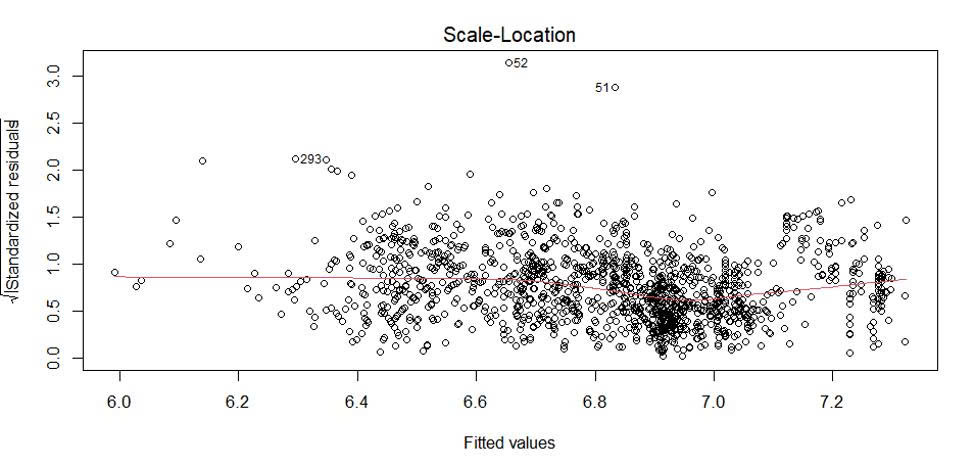
\includegraphics[width=0.88\textwidth]{statisticPros/diag_3_scale_location.jpg}
                \caption{Biểu đồ Scale-Location}
                \label{fig:scale_loc}
            \end{figure}
            \textbf{Nhận xét:} Đường xu hướng màu đỏ tương đối nằm ngang, dao động nhẹ quanh mức $0.6 - 0.85$ và các điểm dữ liệu phân bố khá đều trong dải từ $0.0$ đến $1.5$, không tạo thành hình phễu mở rộng hay thu hẹp rõ rệt dọc theo trục \texttt{Fitted values}. Điều này chứng tỏ giả thiết về phương sai đồng nhất của sai số (\textit{homoscedasticity}) cơ bản được thỏa mãn, chỉ xuất hiện một vài điểm ngoại lai có độ phân tán lớn như điểm 51, 52 và 293.

        \subsubsection{Biểu đồ Residuals vs Leverage (Giá trị dư theo đòn bẩy)}
            \begin{figure}[H]
                \centering
                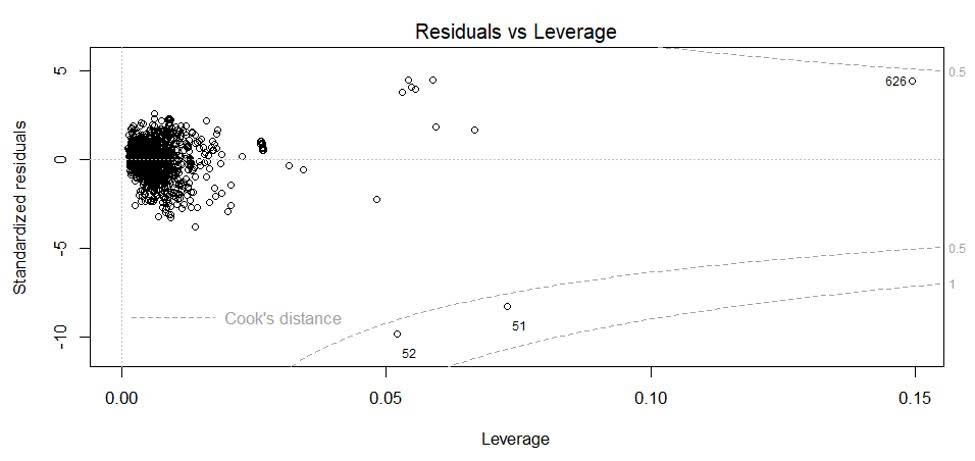
\includegraphics[width=0.88\textwidth]{statisticPros/diag_4_leverage.jpg}
                \caption{Biểu đồ Residuals vs Leverage}
                \label{fig:res_leverage}
            \end{figure}
            \textbf{Nhận xét:} Phần lớn các quan sát tập trung dày đặc ở vùng đòn bẩy thấp ($\text{Leverage} < 0.03$) và nằm hoàn toàn bên trong giới hạn khoảng cách Cook ($\text{Cook's distance} < 0.5$). Đồ thị phát hiện một số điểm có độ ảnh hưởng lớn là điểm 51 và 52 vượt ra ngoài đường giới hạn $0.5$ (nằm sát đường $1$), cùng điểm 626 có giá trị đòn bẩy cao ($\text{Leverage} \approx 0.15$) nhưng vẫn nằm dưới ngưỡng $0.5$. Nhìn chung, không có điểm nào vượt qua ngưỡng nguy hiểm ($\text{Cook's distance} > 1$), chứng tỏ mô hình khá ổn định và không bị bóp méo nghiêm trọng bởi các điểm ngoại lai.

    \subsection{Dự đoán giá trị dựa vào mô hình hồi quy}
        Sử dụng hàm \texttt{predict()} trên Mô hình 3 để tính toán giá trị xung nhịp dự đoán (cả ở dạng logarit và quy đổi ngược về đơn vị thực tế MHz qua hàm mũ $e^x$) và đối chiếu với dữ liệu thực tế:

        \begin{figure}[H]
            \centering
            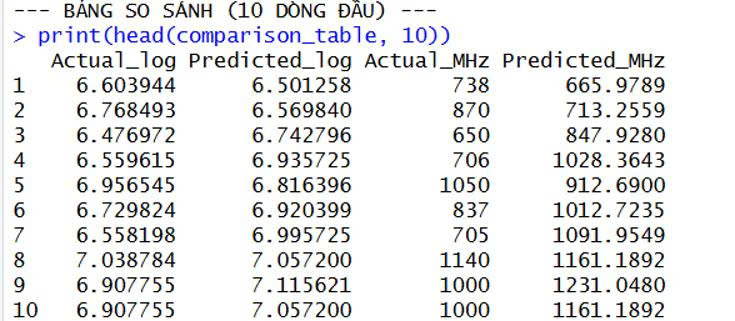
\includegraphics[width=0.85\textwidth]{statisticPros/predict_table.jpg}
            \caption{Bảng so sánh giá trị thực tế và giá trị dự đoán từ Mô hình 3 (10 quan sát đầu)}
            \label{fig:predict_table}
        \end{figure}

        \begin{figure}[H]
            \centering
            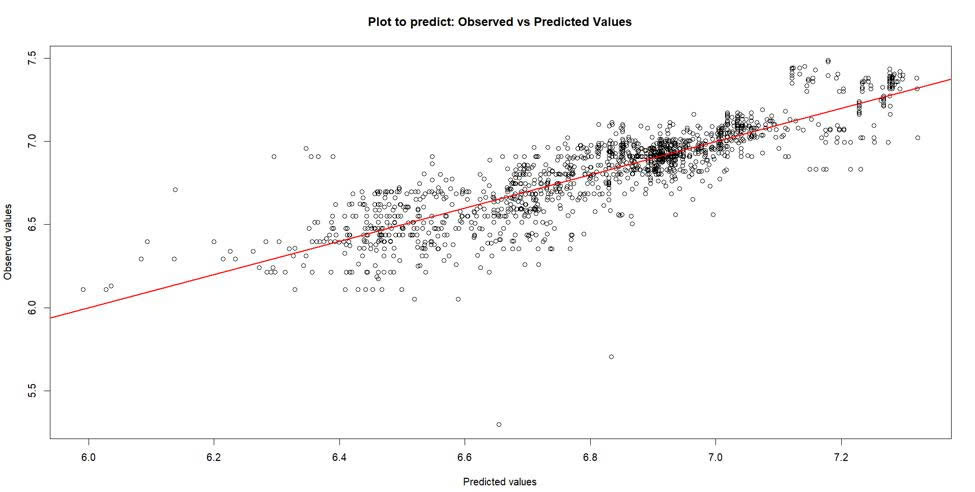
\includegraphics[width=0.88\textwidth]{statisticPros/plot_to_predict.jpg}
            \caption{Đồ thị so sánh giá trị dự đoán (Predicted) và giá trị thực tế (Observed)}
            \label{fig:plot_predict}
        \end{figure}

        \textbf{Đánh giá kết quả dự đoán:} Qua bảng so sánh số liệu (Hình \ref{fig:predict_table}) và đồ thị tương quan dự đoán (Hình \ref{fig:plot_predict}), các điểm quan sát bám khá sát đường xu hướng tuyến tính màu đỏ. Mặc dù mô hình chưa thể tái tạo chính xác tuyệt đối mọi giá trị thực tế, nhưng mức độ sai số nằm trong giới hạn nhỏ và hoàn toàn có thể chấp nhận được. Điều này khẳng định mô hình có độ tin cậy tốt và mang ý nghĩa thống kê cao.